% -------------- TABLA PARA REQUERIMIENTOS FUNCIONALES ---------------- %
% Nomenclatura para la prioridad:
%	MA - Muy Alta
%	A - Alta
%	M - Media
%	B - Baja
%	MB - Muy Baja

\begin{table}[htbp!]
    \begin{requerimientos}

%-----------------------------------------------------Requerimeintos de Usuario-----------------------------------------------------------

        \FRitem{SP1-U1}{Registrar Unidad de Aprendizaje}{El usuario Docente puede registrar los datos de las Unidades de Aprendizaje, de acorde a la entidad Unidad de Aprendizaje del \hyperref[MDD]{Modelo de Datos},  que contiene el Mapa Curricular.}{A}{Origen}
        \label{SP1-U1}

        \FRitem{SP1-U2}{Registrar Usuarios de la Unidad Académica}{El sistema debe permitirle al Jefe de Innovación Educativa registrar a los usuarios integrantes de la Unidad Académica a la que este pertenece (Analista y Docente).}{A}{Origen}
        \label{SP1-U2}

        \FRitem{SP1-U3}{Consultar Mapa Curricular }{El sistema debe permitirle al usuario Docente visualizar la totalidad de los contenidos del Mapa Curricular registrados.}{A}{Origen}
        \label{SP1-U3}

        \FRitem{SP1-U4}{Finalizar Carga Mapa Curricular}{El sistema debe permitirle al usuario Docente indicar cuando ya a finalizado el registro de todas las Unidades de Aprendizaje que contiene el Mapa  Curricular.}{A}{Origen}
        \label{SP1-U4}

        \FRitem{SP1-U5}{Consultar Usuarios de la Unidad Académica}{El sistema debe permitirle al Jefe de Innovación Educativa consultar los usuarios integrantes de la Unidad Académica a la que este pertenece.}{A}{Origen}
        \label{SP1-U5}

        \FRitem{SP1-U6}{Validar congruencia en el Mapa Curricular}{ Si algunos de los datos ingresados se contradicen el sistema no permitirá que se guarden hasta resolver el conflicto.}{A}{Origen}
        \label{SP1-U6}

        \FRitem{SP1-U7}{Enviar Comentarios}{ El Sistema debe permitirle a los Usuarios del Departamento de Innovación Educativa enviar comentarios de corrección sobre el Mapa Curricular una vez que el registro haya finalizado.}{A}{Origen}
        \label{SP1-U7}

        \FRitem{SP1-U8}{Visualizar Comentarios}{ El Sistema debe permitirle al Usuario Docente visualizar comentarios hechos al Mapa Curricular, tanto por el Departamento de Innovación Educativa como por la DES.}{A}{Origen}
        \label{SP1-U8}

        \FRitem{SP1-U9}{Modificar Unidad de Aprendizaje}{El sistema debe permitirle al usuario Docente modificar los datos de las Unidades de Aprendizaje registradas.}{M}{Origen}
        \label{SP1-U9}

        \FRitem{SP1-U10}{Eliminar Unidad de Aprendizaje}{El sistema debe permitirle al usuario Docente eliminar las Unidades de Aprendizaje registradas.}{M}{Origen}
        \label{SP1-U10}

        \FRitem{SP1-U11}{Guardar Avances del Mapa Curricular}{El sistema debe permitirle al usuario Docente guardar las Unidades de Aprendizaje que este vaya registrando.}{M}{Origen}
        \label{SP1-U11}

        \FRitem{SP1-U12}{Aprobar Mapa Curricular}{el Sistema debe permitirle al Usuario Jefe  de Innovación Educativa aprobar el Mapa Curricular una vez que el registro haya finalizado.}{M}{Origen}
        \label{SP1-U12}

        \FRitem{SP1-U13}{Revisar Mapa Curricular}{el Sistema debe permitirle al Usuario Analista revisar el Mapa Curricular una vez que el registro haya finalizado.}{B}{Origen}
        \label{SP1-U13}

        \FRitem{SP1-U14}{Modificar Usuarios de la Unidad Académica}{El sistema debe permitirle al Jefe de Innovación Educativa modificar la información general de los usuarios integrantes de la Unidad Académica a la que este pertenece.}{B}{Origen}
        \label{SP1-U14}

        \FRitem{SP1-U15}{Eliminar Usuarios de la Unidad Académica}{El sistema debe permitirle al Jefe de Innovación Educativa eliminar a cualquier usuario integrante de la Unidad Académica a la que este pertenece.}{B}{Origen}
        \label{SP1-U15}

        \FRitem{SP1-U16}{Notificar al Usuario}{el Sistema informará al los usuarios el estatus de las tareas a las que están asignados.}{B}{Origen}
        \label{SP1-U16}
    \end{requerimientos}
\caption{Requerimientos  de Usuario del subproceso de elaboración del Mapa Curricular}
\label{tbl:RFUA}
\end{table}
%------------------------------------------------------Requerimeintos Funcionales-----------------------------------------------------------

\begin{table}[htbp!]
	\begin{requerimientos}
        \FRitem{SP1-F1}{Registrar Unidad de Aprendizaje}{El sistema debe permitir que el usuario de tipo "Docente" registre los datos de las Unidades de Aprendizaje, de acorde a la entidad Unidad de Aprendizaje del \hyperref[MDD]{Modelo de Datos}.}{A}{Origen}
        \label{SP1-F1}

        \FRitem{SP1-F2}{Registrar Usuarios de la Unidad Académica}{El sistema debe permitir que el usuario de tipo "Jefe de Innovación Educativa" registre a los usuarios integrantes de la Unidad Académica a la que éste pertenece (Analista y Docente).}{A}{Origen}
        \label{SP1-F2}

        \FRitem{SP1-F3}{Consultar Mapa Curricular }{El sistema debe permitir que el usuario de tipo "Docente" visualice todos los registros existentes del Mapa curricular al que está asignado.}{A}{Origen}
        \label{SP1-F3}

        \FRitem{SP1-F4}{Finalizar Carga Mapa Curricular}{El sistema debe permitir que el usuario de tipo "Docente" indique que ha finalizado el registro de todas las Unidades de Aprendizaje que contiene el Mapa  Curricular al que está asignado.}{A}{Origen}
        \label{SP1-F4}

        \FRitem{SP1-F5}{Consultar Usuarios de la Unidad Académica}{El sistema debe permitir que el usuario de tipo "Jefe de Innovación Educativa" consulte los usuarios integrantes de la Unidad Académica a la que éste pertenece.}{A}{Origen}
        \label{SP1-F5}

        \FRitem{SP1-F6}{Validar congruencia en el Mapa Curricular}{ Si algunos de los datos ingresados se contradicen el sistema no permitirá que se guarden hasta resolver el conflicto.}{A}{Origen}
        \label{SP1-F6}

        \FRitem{SP1-F7}{Enviar Comentarios}{ El sistema debe permitir que los usuarios de tipo "Analista" y  "Jefe de Innovación Educativa" envien comentarios de corrección sobre el Mapa Curricular una vez que el usiario de tipo "Docente" haya finalizado el registro.}{A}{Origen}
        \label{SP1-F7}

        \FRitem{SP1-F8}{Visualizar Comentarios}{ El sistema debe permitir que el usuario de tipo "Docente" visualice los comentarios hechos a lastareas que este asignado, tanto los hechos por el Departamento de Innovación Educativa como por la DES.}{A}{Origen}
        \label{SP1-F8}

        \FRitem{SP1-F9}{Modificar Unidad de Aprendizaje}{El sistema debe permitir que el usuario de tipo "Docente" modifique cualquier dato de las Unidades de Aprendizaje que contiene el Mapa Curricular al que está asignado.}{M}{Origen}
        \label{SP1-F9}

        \FRitem{SP1-F10}{Eliminar Unidad de Aprendizaje}{El sistema debe permitir que el usuario de tipo "Docente" elimine las Unidades de Aprendizaje registradas.}{M}{Origen}
        \label{SP1-F10}

        \FRitem{SP1-F11}{Guardar Avances del Mapa Curricular}{El sistema debe permitirle al usuario Docente guardar las Unidades de Aprendizaje que éste vaya registrando.}{M}{Origen}
        \label{SP1-F11}

        \FRitem{SP1-F12}{Aprobar Mapa Curricular}{El sistema debe permitir que el usuario de tipo "Jefe de Innovación Educativa" apruebe el Mapa Curricular de la Unidad Académica a la que éste pertenece una vez que el usuario de tipo "Analista" haya finalizada la revisión.}{M}{Origen}
        \label{SP1-F12}

        \FRitem{SP1-F13}{Revisar Mapa Curricular}{El sistema debe permitir que el usuario de tipo "Analista" revise el Mapa Curricular al que esta asignado una vez que el usuario de tipo "Docente" haya finalizada el registro.}{B}{Origen}
        \label{SP1-F13}

        \FRitem{SP1-F14}{Modificar Usuarios de la Unidad Académica}{El sistema debe permitir que el usuario de tipo "Jefe de Innovación Educativa" modifique la información general de los usuarios integrantes de la Unidad Académica a la que éste pertenece.}{B}{Origen}
        \label{SP1-F14}

        \FRitem{SP1-F15}{Eliminar Usuarios de la Unidad Académica}{El sistema debe permitir que el usuario de tipo "Jefe de Innovación Educativa" elimine a cualquiera de los usuarios integrantes de la Unidad Académica a la que éste pertenece.}{B}{Origen}
        \label{SP1-F15}

        \FRitem{SP1-F16}{Notificar al Usuario}{El sistema informará al los usuarios el estatus de las tareas a las que están asignados.}{B}{Origen}
        \label{SP1-F16}
    \end{requerimientos}
    \caption{Requerimientos funcionales del subproceso de elaboración del Mapa Curricular}
    \label{tbl:RFUA}
\end{table}

% \begin{figure}[htbp]
%     \begin{center}
%         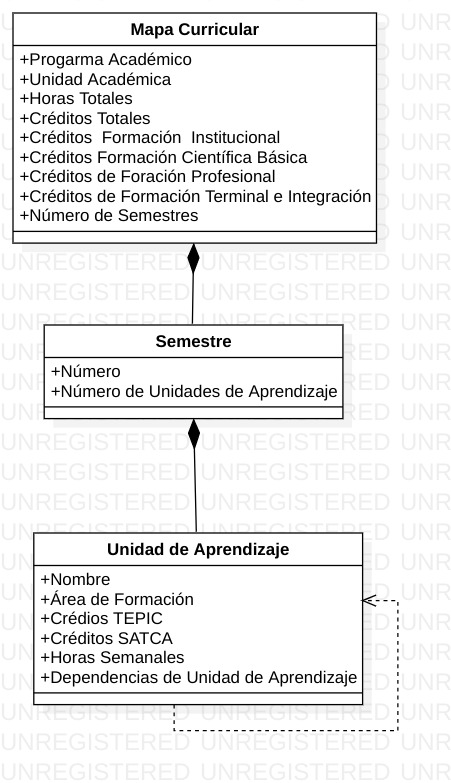
\includegraphics[width=.50\textwidth]{C2-DR/SP4/Image/ModeloDeDatosMC}
%         \label{fig:MD}
%         \caption{Modelo de Datos Subproceso para la  Carga del Mapa Curricular}
%     \end{center}
% \end{figure}

% \begin{figure}[htbp]
% 	\begin{center}
% 		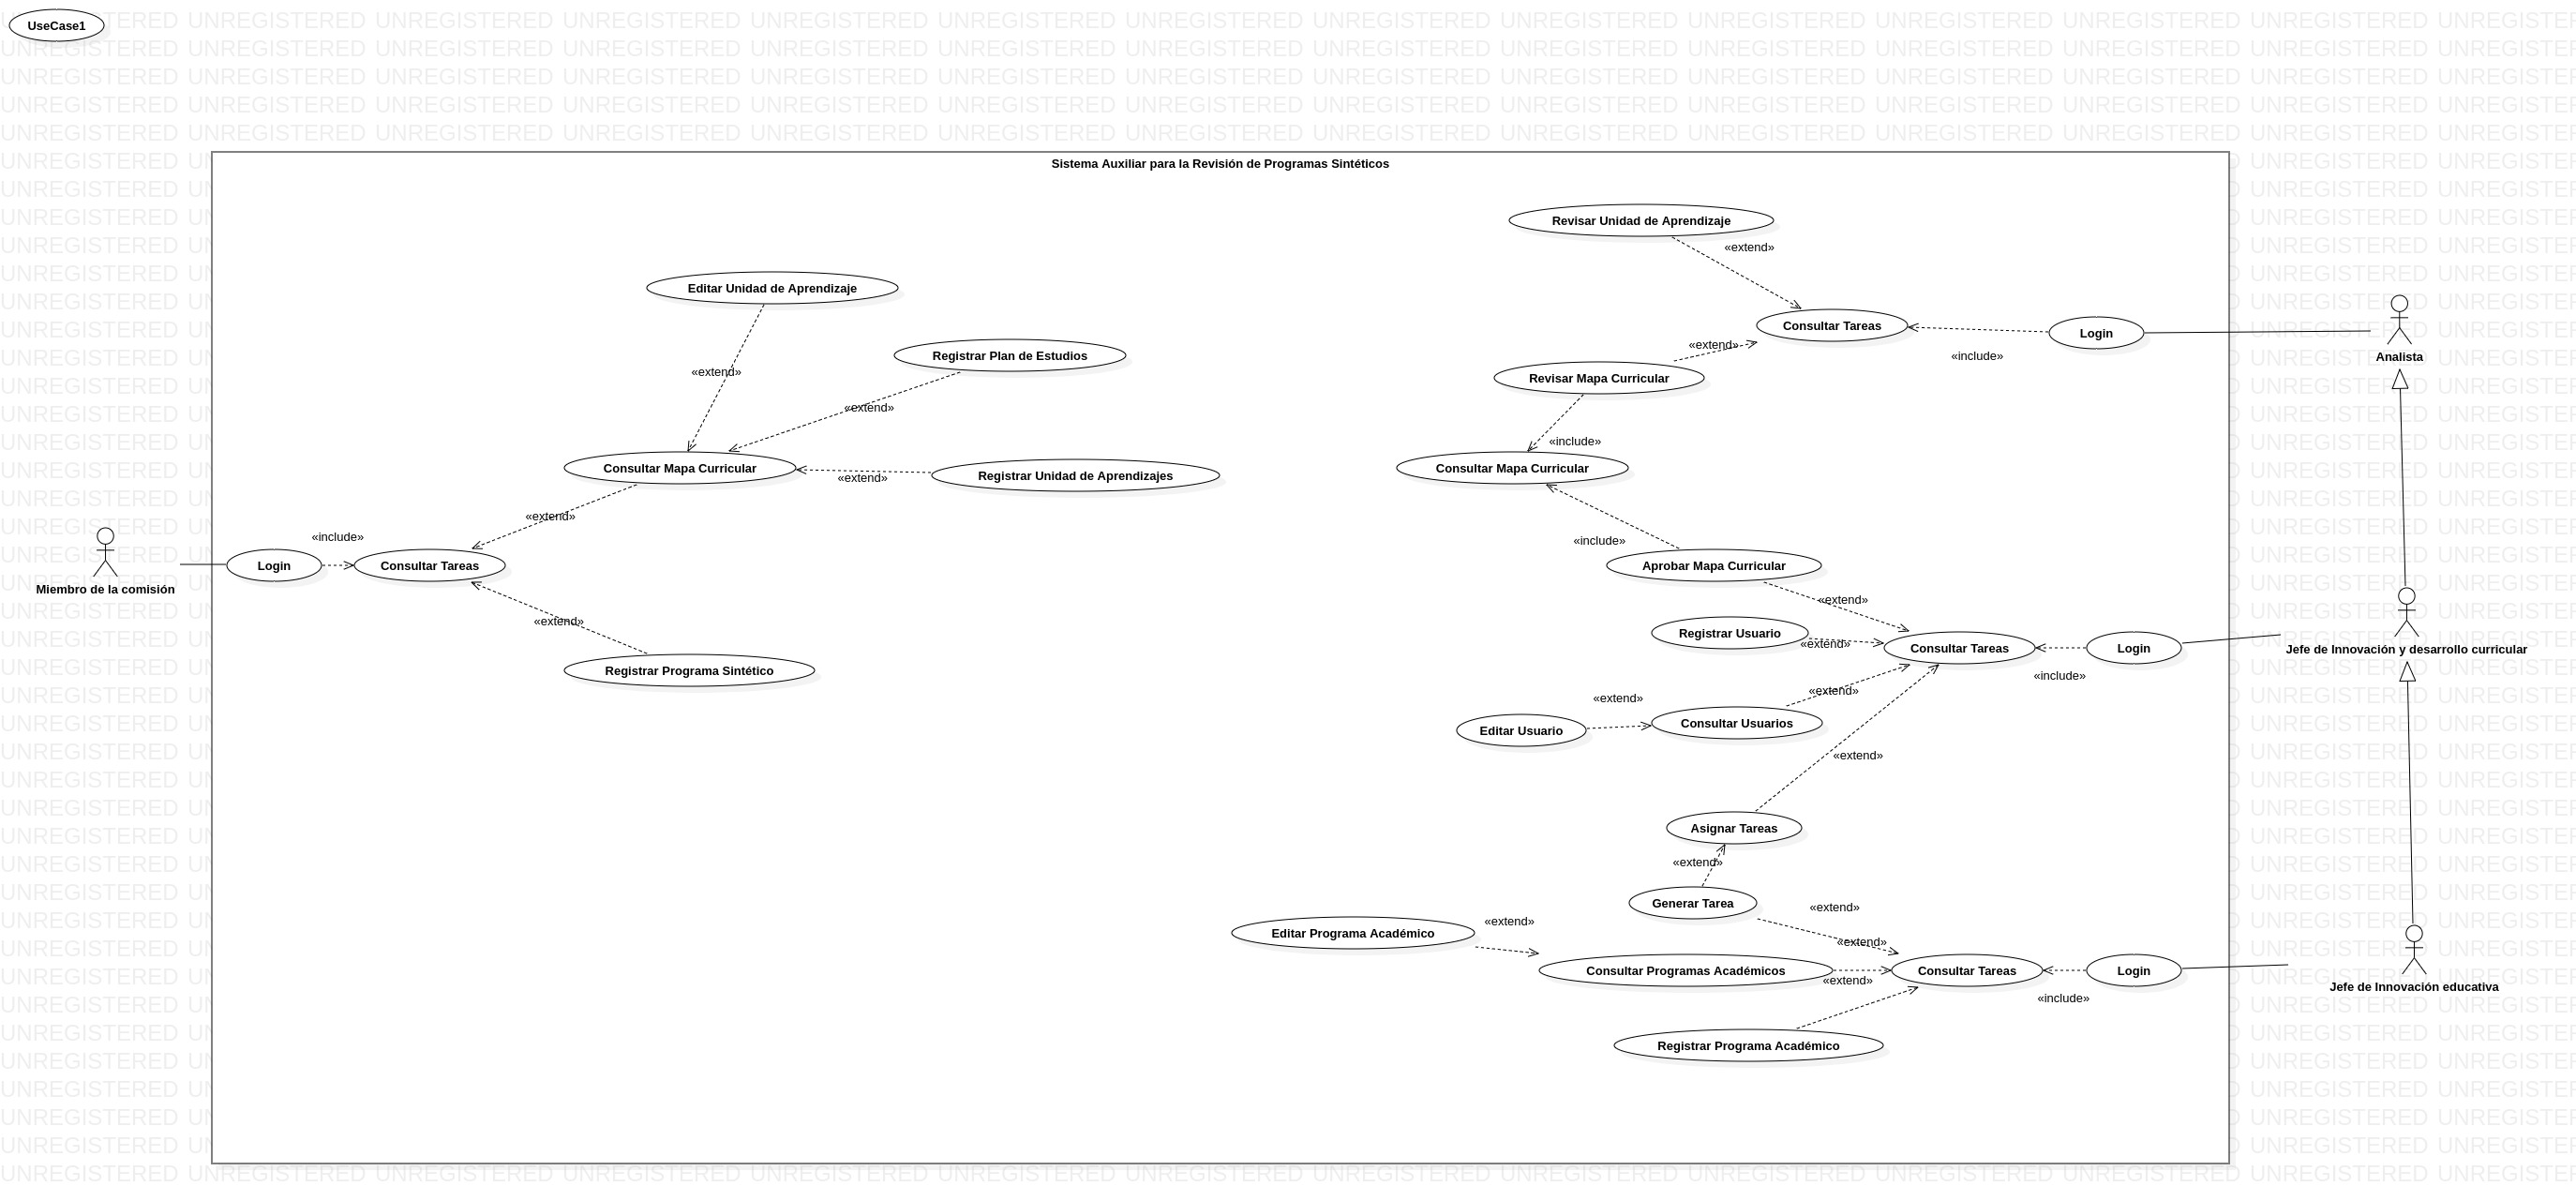
\includegraphics[width=.95\textwidth]{C2-DR/SP4/Image/CasosDeUso}
% 		\caption{Casos de Uso Subproceso para la  Carga del Mapa Curricular}
% 		\label{CU-SP4}
% 	\end{center}
% \end{figure}

% \begin{center}
% 	\begin{tabular}{|c|c|c|c|}
% 		\hline
% 		ID & Caso de uso & Requerimientos & Encargado \\ \hline
%         1 & Registrar Mapa Curricular & \hyperref[RM1]{RM1} & Josué \\ \hline
%         2 & Guardar Mapa Curricular & \hyperref[RM4]{RM4} & Andrés \\ \hline
%         3 & Consultar Mapa Curricular & \hyperref[RM5]{RM5} & Arturo \\ \hline
% 		4 & Editar Información General & \hyperref[RM6]{RM6} & Josué \\ \hline
%         5 & Finalizar Mapa Curricular & \hyperref[RM3]{RM3} & Josué \\ \hline
%         6 & Aprobar Mapa Curricular & \hyperref[RM11]{RM11} & Andrés \\ \hline
%         7 & Registrar Unidades de Aprendizaje & \hyperref[RM2]{RM2} & Arturo \\ \hline
%         8 & Editar Unidades de Aprendizaje & \hyperref[RM8]{RM8} & Andrés \\ \hline
%         9 & Eliminar Unidades de Aprendizaje & \hyperref[RM7]{RM7} & Arturo \\ \hline
%         10 & Registrar Dependencias & \hyperref[RM9]{RM9} & Andrés \\ \hline
%         11 & Editar Dependencias & \hyperref[RM9]{RM9} & Josué \\ \hline
%         12 & Eliminar Dependencias & \hyperref[RM9]{RM9} & Arturo \\ \hline
%         13 & Visualizar Comentarios & \hyperref[RM13]{RM13} & Josué \\ \hline
%         14 & Enviar Comentarios & \hyperref[RM12]{RM12} & Andrés \\ \hline
%     \end{tabular}
% \end{center}
